\chapter{Introducción}

\section{Enfermedades neurodegenerativas y neurciencia}
\subsection{Enfermedades neurodegenerativas}
Hoy en día las enfermedades neurodegenerativas están tomando cada vez más relevancia en
el ámbito de la investigación, ya que constituyen una de las principales causes de mortalidad
en España. Es de gran importancia su diagnóstico temprano, teniendo en cuenta el papel
crucial de los neurotransmisores, para así poder llevar a cabo un tratamiento lo más eficaz
posible.\\

\begin{figure}
	\centering
	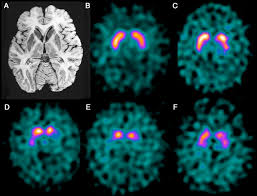
\includegraphics[width=0.5\linewidth]{imagenes/act dopaminergica imagen spect}
	\caption{Actividad dopaminérgica en áreas neuronales específicas afectadas por la enfermedad de Parkinson.}
	\label{fig:act-dopaminergica-imagen-spect}
\end{figure}


Entre ellas destacan el Parkinson (EP), el Alzheimer (EA) y la esclerosis lateral amiotrófica (ELA),
basadas principalmente en la perdida progresiva de células en áreas neuronales específicas. La
EP afecta a las neuronas dopaminérgicas en la sustancia negra, reduciendo los niveles de
dopamina, y a los ganglios basales y llevando a la disfunción del sistema dopaminérgico
cerebral. Esto deriva en la aparición del deterioro cognitivo y problemas de coordinación y
movimiento entre otros. En el caso de la EA, ciertas regiones del cerebro presentan una
disminución de las neuronas colinérgicas, produciendo perdidas en la capacidad de
comunicación y alteraciones en la memoria. En otros casos como la ELA o la enfermedad de
Huntington también deriva en una progresiva parálisis muscular en el primer caso y
movimientos involuntarios en el segundo. \cite{jordan2003avances}\\

Para llegar a entender los efectos producidos por estas enfermedades, hay que poner el foco
en los neurotransmisores afectados por las mismas. EL estudio y análisis de estas variables
permite encontrar un tratamiento que ralentice el avance hacia el declive cognitivo. Por
ejemplo, en el caso del Alzheimer se han desarrollado fármacos que potencian la síntesis de la
acetilcolina, y también inhiben su catabolismo y activan sus receptores. Para el Parkinson, la
levodopa es el tratamiento más eficaz para incrementar la síntesis de la levodopa y para
activar sus receptores. Aún así, tras años de investigación en este ámbito, ningún fármaco ni
tratamiento ha llegado a detener la progresión de estas enfermedades.\\


\subsection{Enfermedad de Parkinson (EP)}

La EP afecta al 1\% de la población mayor de 50 años y tiene una duración estimada de entre 10
y 20 años, afectando de forma progresiva a los pacientes hasta llegar a la invalidez completa. Este trastorno tiene diversas causas:
\begin{itemize}
	\item Alteraciones metabólicas y farmacológicas que afectan a la neurotransmisión de dopamina de los ganglios basales y a las neuronas dopaminérgicas de la sustancia negra.
	\item Pérdida de neuronas estriadas.
	\item Formación de inclusiones celulares llamadas cuerpos de Lewy.
\end{itemize}

\begin{figure}[h]
\centering
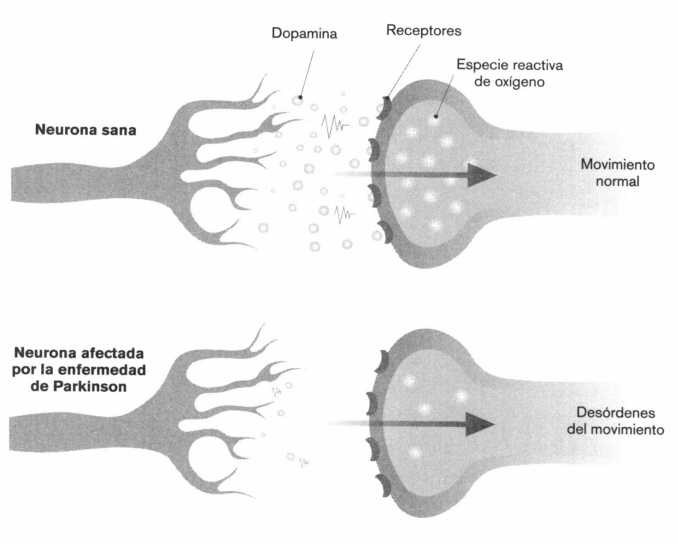
\includegraphics[width=0.5\textwidth]{imagenes/Reducción de transmición dopaminérgica}
\caption{Reducción de la transmisión dopaminérgica de las neuronas afectadas por el Parkinson.}
\label{fig:scan reducción dopamina}
\end{figure}
Entre las principales consecuencias de lo anterior, los pacientes presentas síntomas motores como temblor, rigidez y lentitud de movimientos, pero también no motores como apatía, deterioro cognitivo y síntomas autonómicos. Todo esto afecta drásticamente en la vida de los pacientes. En el caso del Parkinson idiopático (75\% de casos), se distinguen varias fases en función de los indicios detectados: \cite{Elparkin42:online}

\begin{itemize}
	\item Fase inicial con síntomas leves y unilaterales que puede mostrar temblor en
	extremidades superiores entre otros.
	\item Etapa con alteraciones postulares más evidentes y postura encorvada. Aparecen
	síntomas bilaterales.
	\item Se desarrolla incapacidad moderada y alteraciones más pronunciadas, con una dificultad
	de movimiento más resaltado.
	\item Llegando a una fase avanzada de la enfermedad, el individuo requiere asistencia para
	realizar las actividades del día a día debido a la evolución de la incapacidad debida en parte a la
	bradicinesia.
	\item En la última etapa se llega a la incapacidad completa de movimiento.
\end{itemize}

En resumen, a medida que avanza la enfermedad , los problemas motores se generalizan y afectan a ambos lados del cuerpo, mientras la capacidad de procesamiento se deteriora. Todo esto incluye tanto fluctuaciones motoras como no motoras.\cite{martinez2016actualizacion}\\

\subsection{Neurotecnologías}

 La neurociencia y las neurotecnologías han evolucionado mucho desde los descubrimientos de Ramón y Cajal en 1888 hasta los últimos avances en mapas celulares del cerebro humano y en el entendimientos de los circuitos neuronales y la plasticidad cerebral. Sin embargo, hoy en día siguen siendo un gran reto las enfermedades neurológicas, conllevando altos costes y complicaciones. Pero gracias a la combinación de neurociencia con inteligencia artificial y robótica que ofrecen las neurotecnologías modernas, se espera avanzar en la investigación dentro de este ámbito, aunque también habrá que tratar dilemas éticos y morales.\cite{6OFICINA49:online}\\

Existen tres tipos de avances neurotecnológicos: neuroimagen (registro de actividad cerebral), neuromodulación (modificación de señales cerebrales) y neurofeedback (bucle de registro y respuesta de señales). Además, pueden ser tecnologías invasivas, semi-invasivas o no invasivas en función del método de conexión con el sistema nervioso y el riesgo que implican para el paciente.\\

Entra las principales limitaciones debidas a las tecnologías actuales se encuentra: la complejidad de captar la actividad neuronal de forma no invasiva y con alta precisión, y la dificultad de manejar grandes cantidades de datos. Como respuesta, se están intentando desarrollar materiales y técnicas para una mejor resolución y seguridad en el registro de actividad cerebral. Además, gracias al uso de la inteligencia artificial como herramienta para procesar la gran cantidad de información, se puede procesar y entender de manera más eficaz, permitiendo tratamientos más avanzados. Esto permite llevar a cabo tratamientos más efectivos y personalizados para distintas condiciones neurológicas.\\

El principal enfoque de las neurotecnologías es ayudar a personas con discapacidades motoras y sensoriales. Para ello, se están investigando las interfaces cerebro-ordenador que, combinadas con fisioterapia, muestran resultados prometedores para la rehabilitación de extremidades paralizadas. La estimulación de la plasticidad neuronal conseguida debido a los avances en el diseño de neuroprótesis y robots, también facilita la recuperación funcional de los pacientes.  \\

Por otro lado, también se están desarrollando dispositivos que permitan restaurar la audición y la visión, como pueden ser los implantes cocleares, ya utilizados para tratar la sordera, o los implantes de retina, que aun están siendo investigados pero que permitirían recuperar la capacidad visual.\\

Además, hay un campo de investigación centrado en la decodificación cerebral tanto del lenguaje como del pensamiento visual y de los estados emocionales. El objetivo es mejorar la comunicación mediante interfaces cerebro-ordenador de personas con parálisis. Por ejemplo, algunas de las nuevas tecnologías que se están llevando a cabo traducen la actividad cerebral para que pueda ser interpretada por una computadora. También se avanza en reconstruir imágenes visuales observadas y en comprender estados emocionales y niveles de conciencia, útiles tanto para mejorar la calidad del sueño como para tratar trastornos neuropsiquiátricos como la depresión.\\

En cuanto a la realidad virtual, puede llegar a tener un gran potencial en combinación con las interfaces cerebro-ordenador, por ejemplo para trata pacientes tetrapléjicos u para otros fines medico y también en el ámbito de los videojuegos. Además, muchas empresas están realizando importantes inversiones, por lo que a pesar de implicar altos costes se están volviendo cada vez más accesibles. Se espera que en los próximos años estas tecnologías mejoren la capacidad cognitiva y la consciencia, pero también se deberán tratar dilemas legales y éticos, ya que por ejemplo, la privacidad mental y la seguridad de los neurodatos estarán en el punto de mira debido a los riesgos de violaciones de privacidad que pueden venir de la mano de las neurotecnologías y la inteligencia artificial. Por ello, es crucial que haya un consentimiento informado para que los distintos riesgos.\\

En cuanto a los altos costes, estos pueden derivar en diferencias sociales en función del acceso a estas tecnologías. También es muy importante tener en cuenta los efectos adversos a largo plazo que pueden tener además de todos sus beneficios y mejoras en el aprendizaje y la memoria, siendo crucial una regulación ética y legal estricta.\\

Diversos organismos internacionales y nacionales están estableciendo marcos legales que protejan lo conocido como neuroderechos. Las Iniciativas impulsadas por grupos como la UNESCO o la OCDE han hecho resaltar la necesidad de una regulación global, mientras que en Europa aun no existe una legislación especifica para las neurotecnologías. Sin embargo, en diversos países como España o Francia ya han incluido los neuroderechos en sus constituciones, avanzando así en la protección de datos neuronales. También se ha reflejado un compromiso Europeo y Español de la promoción de neuroderechos con las declaraciones de León y Valencia.\\

En España, la regulación de las neurotecnologías está enfrentándose a desafíos importantes:
\begin{itemize}
	\item La Agencia Española del Medicamento y Productos Sanitarios (AEMPS)se encarga de supervisar evaluaciones clínicas estrictas, intentando asegurar la seguridad y eficacia de estas tecnologías.
	\item La Red Española de Agencias de Evaluación de Tecnologías Sanitarias (RedETS) gestiona la inclusión de estas tecnologías en la cartera de servicios del Sistema Nacional de Salud.
	\item El Reglamento (UE) 2022/2346 regula las neurotecnologías no invasivas fuera del ámbito clínico, que pide evaluaciones exhaustivas de riesgos y efectos.
\end{itemize}

Desde 2013, se han invertido significativas sumas en proyectos globales de investigación cerebral como BRAIN en EE.UU. y el Proyecto Cerebro Humano en Europa, buscando avanzar en neurotecnologías para comprender mejor la actividad neuronal y su impacto en la cognición. Se enfatiza la creación de infraestructuras científicas y plataformas digitales para facilitar el acceso a datos y herramientas de modelización. La comunidad científica aboga por aumentar la financiación y la colaboración interdisciplinaria para acelerar la aplicación clínica y social de estos avances, destacando la importancia de una regulación ética que promueva la innovación responsable.\\


\subsection{Modelos Predictivos}
No cabe duda que la creación y avance de modelos predictivos para predecir la evolución de la enfermedad de Parkinson, incluido el declive cognitivo, reviste una importancia crucial, permitiendo avanzar en diagnósticos más personalizados y precisos. Actualmente existen diversos modelos predictivos basados en datos clínicos, genéticos y de imagenología, como lo que se han utilizado en el presente estudio, que han demostrado cierto grado de precisión en la predicción de la progresión de la enfermedad.\\

Estos modelos emplean técnicas estadísticas y de aprendizaje automático para analizar grandes conjuntos de datos y extraer patrones y tendencias relevantes. Sin embargo, aún hay desafíos importantes por superar, como la heterogeneidad de la enfermedad y la necesidad de datos longitudinales y multimodales para una predicción más precisa. \cite{Predicti52:online}\\

En este contexto, la inteligencia artificial (IA) emerge como una herramienta prometedora que permitirá avanzar en el diseño de modelos predictivos más precisos y personalizados para la enfermedad de Parkinson. Los algoritmos de IA, como las redes redes de muestreo como puede ser Leaspy,
tienen el potencial de manejar datos complejos y heterogéneos de manera más efectiva, identificando
correlaciones sutiles y no lineales que pueden pasar desapercibidas para los enfoques tradicionales.\\

En resumen, avanzar en el diseño de modelos predictivos para la enfermedad de Parkinson, incluido el
declive cognitivo, es fundamental para mejorar la atención médica y la calidad de vida de los pacientes.
La aplicación de la inteligencia artificial abre nuevas posibilidades para lograr predicciones más precisas
y personalizadas, allanando el camino hacia una atención médica más efectiva y centrada en el paciente.\\

\subsection{Impacto socioeconómico}
La enfermedad de Parkinson tiene un impacto significativo en el ámbito socioeconómico, afectando a los pacientes, a sus familias y a la sociedad en general. Además, cada vez tiene más relevancia debido al constante cambio que sufre el contexto demográfico, caracterizado por el envejecimiento general de la población debido al aumento de la esperanza de vida y a la disminución de la natalidad. Esto tiene crucial importancia ya que el Parkinson afecta principalmente a personas de avanzada edad, viendo como dicho grupo está aumentando considerablemente. Esta tendencia tiene importantes implicaciones para la salud pública y el sistema de atención médica, ya que el envejecimiento de la población se asocia con un mayor riesgo de enfermedades crónicas, discapacidades y necesidades de atención a largo plazo. \cite{GARCIARAMOS2016401}\\

En este contexto, el impacto socioeconómico del Parkinson adquiere una mayor relevancia, ya que afecta a un segmento cada vez mayor de la población. El tratamiento y manejo de esta enfermedad pueden generar una carga económica significativa para los pacientes y sus familias, especialmente en un entorno demográfico en el que un mayor porcentaje de la población está en edad de jubilación y puede tener recursos financieros limitados.\\

La enfermedad de Parkinson en España genera unos costes importantes, que llegan a alcanzar los 17.000 euros anuales por paciente. Los costes directos, principalmente los tratamientos médicos, llegan a una media de 8.640 euros cada seis meses, de los que 1.456 euros se destinan a medicamentos dopaminérgicos \cite{GARCIARAMOS2016401}. Los costes indirectos, como la pérdida de productividad por jubilación anticipada, aumentan hasta los 6.691 euros por persona en tres meses. Las terapias avanzadas, como la estimulación cerebral profunda (DBS), tienen un coste a cinco años de 88.104 euros, mientras que la infusión subcutánea continua de apomorfina (ICAS) cuesta 141.393 euros y la infusión intraduodenal de levodopa (ICLI) 233.986 euros. Anualmente, estos tratamientos suponen unos costes de 17.603 euros para la DBS, 28.279 euros para la ICAS y 46.796 euros para la ICLI.\\

Además, los casos de Parkinson han sufrido un fuerte aumento, tal y como se ve en la gráfica de la figura \ref{fig:graf_Park_esp} que representa la evolución del Parkinson en España entre el año 2011 y 2022. \cite{RegParkEsp}\\


\begin{figure}[t]
	\centering
	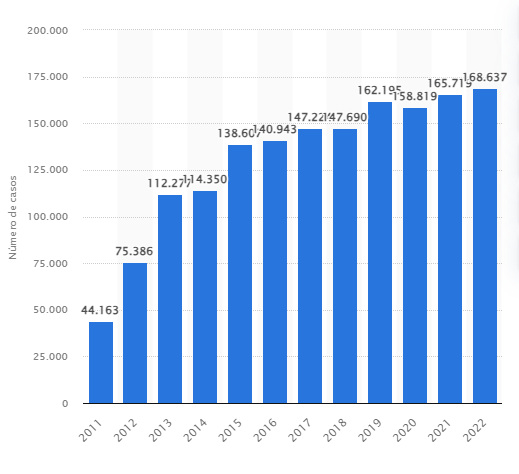
\includegraphics[width=0.7\textwidth]{imagenes/registro_Parkinson}
	\caption{Cifras de casos de Parkinson registrados en España entre los años 2011 y 2022.}
	\label{fig:graf_Park_esp}
\end{figure}

Además, los síntomas motores y no motores del Parkinson pueden afectar la calidad de vida de los pacientes, limitando su participación en actividades sociales y recreativas y generando sentimientos de aislamiento y depresión. Esto puede tener un impacto negativo en el bienestar emocional y social de los pacientes, así como en su capacidad para llevar una vida plena y satisfactoria.\\


\section{Objetivos}
Actualmente, para poder mejorar los tratamientos para las enfermedades neurodegenerativas es necesario poder predecir su aparición y evolución lo antes posible. Se parte de la premisa fundamental de que la detección precoz y el seguimiento preciso de la progresión de la enfermedad son esenciales para mejorar la calidad de vida y ralentizar su avance. Por ello, el objetivo principal de este trabajo es utilizar el entorno de programación para Python llamado \textit{Leaspy}, para predecir la aparición de declive cognitivo en pacientes con enfermedad de Parkinson.\\

\textit{Leaspy} es un paquete de software que facilita el análisis de datos longitudinales como pueden ser los recopilados en la base de datos utilizada, compuesta por observaciones repetidas de un grupo de 423 pacientes a lo largo del tiempo. Esta está formada por datos médicos recopilados de distintas visitas de un grupo de pacientes. \\

Con el programa desarrollado se pretende medir si las predicciones obtenidas utilizando esta herramienta son mas precisas que los resultados obtenidos por otros algoritmos, como el 'Robust Paramétric Disease Progresssion Modeling' (RPDPM). Con esta meta, se calculan diversos parámetros que miden la precisión de los Modelos de Progresión de la Enfermedad (DPMs, por sus siglas en inglés), estimados previamente gracias a funciones características de \textit{Leaspy}. Las prestaciones indican por un lado, la precisión de la trayectoria estimada de la enfermedad en los sujetos, y por otro lado, la exactitud del pronóstico de aparición del declive cognitivo en los pacientes. Todo esto queda reflejado en los parámetros de error absoluto medio (MAE), Área Bajo la Curva (AUC), correlación de de la edad de conversión, correlación de la reserva cognitiva, etc. \\

Además de comparar \textit{Leaspy} con otros métodos de predicción, también se busca comparar los modelos estimados caracterizados por estimar la evolución de la enfermedad en los sujetos a partir de distintos conjuntos de biomarcadores. Por lo que otro de los objetivos de este estudio es encontrar el conjunto de biomarcadores con el que se obtenga una predicción lo más precisa posible de la trayectoria de la enfermedad en los individuos y de la aparición del deterioro cognitivo leve (MCI).\\

En conjunto, este estudio aspira a contribuir significativamente al avance del conocimiento en la estimación de modelos de progresión de la enfermedad de Parkinson, así como a comprender más a fondo el progreso de este tipo de enfermedades.


\section{Estructura del documento}

A continuación y para facilitar la lectura del documento, se detalla el contenido de cada capítulo.

\begin{itemize}
\item En el capítulo 1 se realiza una introducción.
\item En el capítulo 2 se hace un repaso de distintos recursos cruciales para esta investigación.
\item En el capítulo 3 se nombran las distintas herramientas y materiales utilizados en este trabajo.
\item En el capítulo 4 se explica el algoritmo desarrollado. 
\item En el capítulo 5 se muestran los resultados obtenidos y se discuten.
\item En el capítulo 6 se concluye el trabajo y se reflejan los pasos futuros.
\end{itemize}
